\documentclass[aspectratio=169]{beamer}

% ── Theme & Colours ──────────────────────────────────────────────────────────
\usetheme{Madrid}
\usecolortheme{default}

\definecolor{navyblue}{RGB}{26,31,54}
\definecolor{electricblue}{RGB}{79,110,247}
\definecolor{lightblue}{RGB}{220,230,255}
\definecolor{successgreen}{RGB}{34,197,94}
\definecolor{warnorange}{RGB}{245,158,11}
\definecolor{softgray}{RGB}{248,249,252}

\setbeamercolor{palette primary}{bg=navyblue, fg=white}
\setbeamercolor{palette secondary}{bg=electricblue, fg=white}
\setbeamercolor{palette tertiary}{bg=navyblue!80, fg=white}
\setbeamercolor{palette quaternary}{bg=navyblue, fg=white}
\setbeamercolor{structure}{fg=navyblue}
\setbeamercolor{section in toc}{fg=navyblue}
\setbeamercolor{frametitle}{bg=navyblue, fg=white}
\setbeamercolor{title}{fg=white}
\setbeamercolor{subtitle}{fg=lightblue}
\setbeamercolor{author}{fg=lightblue}
\setbeamercolor{date}{fg=lightblue}
\setbeamercolor{institute}{fg=lightblue}
\setbeamercolor{block title}{bg=electricblue, fg=white}
\setbeamercolor{block body}{bg=lightblue!40, fg=navyblue}
\setbeamercolor{block title alerted}{bg=red!70!black, fg=white}
\setbeamercolor{block body alerted}{bg=red!10, fg=black}
\setbeamercolor{block title example}{bg=successgreen!80!black, fg=white}
\setbeamercolor{block body example}{bg=successgreen!10, fg=black}
\setbeamercolor{itemize item}{fg=electricblue}
\setbeamercolor{itemize subitem}{fg=navyblue!70}
\setbeamercolor{enumerate item}{fg=electricblue}

\setbeamertemplate{itemize item}{\scriptsize\raise1.5pt\hbox{\donotcoloroutermaths$\blacktriangleright$}}
\setbeamertemplate{itemize subitem}{\tiny\raise1.5pt\hbox{\donotcoloroutermaths$\bullet$}}
\setbeamertemplate{navigation symbols}{}
\setbeamertemplate{footline}{
  \leavevmode%
  \hbox{%
    \begin{beamercolorbox}[wd=.30\paperwidth,ht=2.5ex,dp=1.5ex,left,leftskip=1mm]{palette primary}%
      \usebeamerfont{author in head/foot}\insertshortauthor
    \end{beamercolorbox}%
    \begin{beamercolorbox}[wd=.40\paperwidth,ht=2.5ex,dp=1.5ex,center]{palette secondary}%
      \usebeamerfont{title in head/foot}\insertshorttitle
    \end{beamercolorbox}%
    \begin{beamercolorbox}[wd=.30\paperwidth,ht=2.5ex,dp=1.5ex,right,rightskip=1mm]{palette primary}%
      \usebeamerfont{date in head/foot}\insertframenumber{} / \inserttotalframenumber
    \end{beamercolorbox}%
  }
}

% ── Packages ─────────────────────────────────────────────────────────────────
\usepackage{amsmath,amssymb}
\usepackage{graphicx}
\usepackage{booktabs}
\usepackage{array}
\usepackage{colortbl}
\usepackage{xcolor}
\usepackage{tikz}
\usetikzlibrary{shapes.geometric, arrows.meta, positioning, fit, backgrounds, shadows.blur}
\usepackage{tcolorbox}
\tcbuselibrary{skins,breakable}
\usepackage{pgfplots}
\pgfplotsset{compat=1.18}
\usepackage{multicol}

\hbadness=10000
\vbadness=10000
\hfuzz=10pt
\vfuzz=200pt

% ── Shared tcolorbox styles ───────────────────────────────────────────────────
% Blue box (primary content)
\tcbset{
  bluebox/.style={colback=electricblue!12, colframe=electricblue,
    fonttitle=\small\bfseries, boxrule=1.2pt, left=4pt, right=4pt,
    top=3pt, bottom=3pt},
  greenbox/.style={colback=successgreen!10, colframe=successgreen!70!black,
    fonttitle=\small\bfseries, boxrule=1.2pt, left=4pt, right=4pt,
    top=3pt, bottom=3pt},
  orangebox/.style={colback=warnorange!12, colframe=warnorange,
    fonttitle=\small\bfseries, boxrule=1.2pt, left=4pt, right=4pt,
    top=3pt, bottom=3pt},
  redbox/.style={colback=red!8, colframe=red!65!black,
    fonttitle=\small\bfseries, boxrule=1.2pt, left=4pt, right=4pt,
    top=3pt, bottom=3pt},
  navybox/.style={colback=navyblue!8, colframe=navyblue,
    fonttitle=\small\bfseries, boxrule=1.2pt, left=4pt, right=4pt,
    top=3pt, bottom=3pt},
}

% ── TikZ Styles ──────────────────────────────────────────────────────────────
\tikzset{
  component/.style={rectangle, rounded corners=4pt, draw=navyblue, thick,
    fill=lightblue!60, text=navyblue, font=\small\bfseries,
    minimum height=0.7cm, minimum width=2.2cm, align=center},
  arrow/.style={-Stealth, thick, color=electricblue},
  flow/.style={rectangle, rounded corners=3pt, draw=navyblue!70, thick,
    fill=white, text=navyblue, font=\footnotesize, align=center,
    minimum height=0.6cm, minimum width=1.8cm},
}

% ── Metadata ─────────────────────────────────────────────────────────────────
\title[SecureFileShare]{Secure Decentralised File Sharing}
\subtitle{Using Blockchain \& IPFS}
\author[IT352 Project]{Aadharsh~Ramachandran and Paluvadi~Dinesh~Manideep}
\institute[Thakur / Universal College]{IT352 Information Assurance and Security Midsemester Project Evaluation}


% =============================================================================
\begin{document}
% =============================================================================

% ── Title Slide ───────────────────────────────────────────────────────────────
\begin{frame}[plain]
\begin{tikzpicture}[remember picture, overlay]
  \fill[navyblue] (current page.north west) rectangle (current page.south east);
  \fill[electricblue, opacity=0.18]
    (current page.north east)
    .. controls +(-3,-2) and +(2,2) ..
    ([xshift=-3cm]current page.east)
    -- (current page.south east) -- cycle;
\end{tikzpicture}
\vspace{0.4cm}
\titlepage
\end{frame}

% ── Outline ───────────────────────────────────────────────────────────────────
\begin{frame}{Presentation Outline}
\begin{tcolorbox}[navybox, title=\textbf{Outline}]
\small
\begin{enumerate}
  \item Introduction \& Problem Statement
  \item Objectives
  \item Novel Contributions
  \item Methodology \& Algorithm
  \item System Architecture
  \item Results \& Analysis
  \item Future Work
\end{enumerate}
\end{tcolorbox}
\end{frame}

% =============================================================================
\section{Introduction \& Problem Statement}
% =============================================================================

\begin{frame}{Introduction --- The Digital Storage Crisis}
\begin{tcolorbox}[redbox, title=\textbf{Core Problem}]
\small
Traditional file sharing systems rely on central servers that are single points of failure ---
vulnerable to data breaches, unauthorized access, and provider misuse. They offer no
cryptographic guarantees over who can access files, for how long, or whether data is truly
deleted when requested --- fundamental, unresolved security risks that grow with every
terabyte stored.
\end{tcolorbox}
\vspace{0.18cm}
\begin{tcolorbox}[bluebox, title=\textbf{Limitations of Centralised Storage}]
\scriptsize
\begin{columns}[t]
\column{0.48\textwidth}
\begin{itemize}
  \item \textbf{Single Point of Failure} --- one breach exposes everything
  \item \textbf{Third-Party Dependency} --- loss of data ownership
  \item \textbf{No Tamper Evidence} --- silent data manipulation possible
\end{itemize}
\column{0.48\textwidth}
\begin{itemize}
  \item \textbf{High Operational Costs} --- centralised infrastructure scales poorly
  \item \textbf{Availability Issues} --- server downtime = inaccessible data
  \item \textbf{Privacy Violations} --- provider retains unilateral access
\end{itemize}
\end{columns}
\end{tcolorbox}
\end{frame}

\begin{frame}{Problem Statement}
\begin{tcolorbox}[redbox, title={\textbf{Problem Statement}}]
\small
How can organisations securely share confidential files over an untrusted network
\textbf{without relying on any central authority}, while simultaneously guaranteeing
\textbf{data integrity}, \textbf{fine-grained cryptographic access control},
\textbf{legal compliance (GDPR)}, and \textbf{mathematical verifiability of access}?
\end{tcolorbox}
\vspace{0.2cm}
\begin{columns}[t]
\column{0.48\textwidth}
\begin{tcolorbox}[bluebox, title=\textbf{What Existing Solutions Miss}]
\small
\begin{itemize}
  \item No ZKP-based privacy-preserving identity verification
  \item Rigid access control (all-or-nothing permissions)
\end{itemize}
\end{tcolorbox}
\column{0.48\textwidth}
\begin{tcolorbox}[greenbox, title=\textbf{What Existing Solutions Miss}]
\small
\begin{itemize}
  \item GDPR ``Right to Erasure'' vs.\ blockchain immutability paradox
  \item Permissions do not expire automatically
  \item Scalability degrades with large file volumes
\end{itemize}
\end{tcolorbox}
\end{columns}
\end{frame}

% =============================================================================
\section{Objectives}
% =============================================================================

\begin{frame}{Research Objectives}
\begin{columns}[t]
\column{0.48\textwidth}
\begin{tcolorbox}[redbox, title=\textbf{Security Objectives}]
\scriptsize
\begin{itemize}
  \item[\textbf{O1}] Encrypt files with \textbf{AES-256-GCM} before any storage
  \item[\textbf{O2}] Verify chunk integrity via \textbf{SHA-256} hashing
  \item[\textbf{O3}] Authenticate users via \textbf{Groth16 ZKP} without revealing credentials
  \item[\textbf{O4}] Implement \textbf{CP-ABE} for policy-driven key management
  \item[\textbf{O5}] Achieve \textbf{GDPR compliance} (Articles 17 \& 20) in Web3
\end{itemize}
\end{tcolorbox}
\column{0.48\textwidth}
\begin{tcolorbox}[bluebox, title=\textbf{Storage Objectives}]
\scriptsize
\begin{itemize}
  \item[\textbf{O6}] Store encrypted chunks on \textbf{IPFS} with CID-based addressing
  \item[\textbf{O7}] Register file metadata immutably on \textbf{Ethereum blockchain}
  \item[\textbf{O8}] Implement \textbf{sharding} for large-file fault tolerance
\end{itemize}
\end{tcolorbox}
\vspace{0.15cm}
\begin{tcolorbox}[greenbox, title=\textbf{Governance Objectives}]
\scriptsize
\begin{itemize}
  \item[\textbf{O9}] Automate access control via \textbf{Smart Contracts}
  \item[\textbf{10}] Enforce \textbf{time-bound permissions} using \texttt{block.timestamp}
\end{itemize}
\end{tcolorbox}
\end{columns}
\end{frame}

% =============================================================================
\section{Novel Contributions}
% =============================================================================

\begin{frame}{Four Novel Contributions}
\begin{columns}[T]
\column{0.48\textwidth}
\begin{tcolorbox}[bluebox, title=\textbf{N1: Zero-Knowledge Proofs (ZKP)},
  height=5.8cm, valign=top]
\scriptsize
\textbf{Circuit:} \texttt{fileIntegrity.circom}\\
\textbf{Protocol:} Groth16 over BN128 curve\\[5pt]
\textbf{What it proves: Proves encrypted chunks match original file hash
▶ Blockchain verifies file validity without seeing content} \\[5pt]
\textbf{Verified by:} \texttt{ZKPVerifier.sol} at download time\\[5pt]
\textbf{Impact:} Privacy-preserving identity; zero information leakage
\end{tcolorbox}
\column{0.48\textwidth}
\begin{tcolorbox}[greenbox, title=\textbf{N2: Attribute-Based Encryption (ABE)},
  height=5.8cm, valign=top]
\scriptsize
\textbf{Scheme:} Ciphertext-Policy ABE via Shamir SSS on BN128 field\\[5pt]
\textbf{Policy example:} \texttt{role:doctor AND org:hospital}\\[5pt]
\textbf{Mechanism:} AES key split into shares; each encrypted with
HKDF-derived per-attribute key from master secret\\[5pt]
\textbf{Impact:} Cryptographic (not just policy) enforcement of access
\end{tcolorbox}
\end{columns}
\end{frame}

\begin{frame}{Four Novel Contributions}
\begin{columns}[T]
\column{0.48\textwidth}
\begin{tcolorbox}[orangebox, title=\textbf{N3: Time-Bound Permissions},
  height=5.8cm, valign=top]
\scriptsize
\textbf{Contract:} \texttt{TimeBoundPermissions.sol}\\[5pt]
\textbf{Mechanism:} \texttt{block.timestamp + durationSeconds} enforced
natively on Ethereum\\[5pt]
\textbf{Features:} Grant, extend, revoke, auto-expire \& batch cleanup
of expired permissions\\[5pt]
\textbf{Impact:} Self-destructing access rights --- no manual revocation
\end{tcolorbox}
\column{0.48\textwidth}
\begin{tcolorbox}[redbox, title=\textbf{N4: GDPR Compliance Module},
  height=5.8cm, valign=top]
\scriptsize
\textbf{Paradox solved:} Blockchain immutability vs.\ Art.\,17 right to erasure\\[5pt]
\textbf{Approach:} IPFS unpin $\to$ SQLite PII anonymisation (SHA-256)
$\to$ on-chain \texttt{isDeleted} flag $\to$ \texttt{ErasureFulfilled} event\\[5pt]
\textbf{Art.\,20:} Full JSON data export from SQLite audit trail\\[5pt]
\textbf{Impact:} First hybrid Web3/GDPR erasure \& export architecture
\end{tcolorbox}
\end{columns}
\end{frame}

% =============================================================================
\section{Methodology}
% =============================================================================

\begin{frame}{Methodology --- 7-Step Algorithm}
\begin{columns}[c]
\column{0.52\textwidth}
\begin{tcolorbox}[navybox, title=\textbf{Algorithm Steps}]
\scriptsize
\begin{enumerate}
  \item[\textbf{S1}] \textbf{Key Generation} ---
    ECDSA P-256 key pair; public key stored on-chain
  \item[\textbf{S2}] \textbf{Encrypt \& Shard} ---
    AES-256-GCM per 64\,KB chunk; SHA-256 hash; CP-ABE key split
  \item[\textbf{S3}] \textbf{IPFS Upload} ---
    Encrypted chunks pinned via Pinata; CIDs returned
  \item[\textbf{S4}] \textbf{Blockchain Register} ---
    \texttt{FileRegistry.uploadFile(CIDs,\,hash)}; Groth16 ZKP verified
  \item[\textbf{S5}] \textbf{Access Grant} ---
    \texttt{grantAccess()} + \texttt{grantTimedAccess()};
    AES key wrapped with recipient public key via ECDH
  \item[\textbf{S6}] \textbf{File Retrieval} ---
    ZKP + ABE + time-bound check; fetch, decrypt, SHA-256 verify
  \item[\textbf{S7}] \textbf{GDPR} ---
    Erasure pipeline
\end{enumerate}
\end{tcolorbox}

\column{0.43\textwidth}
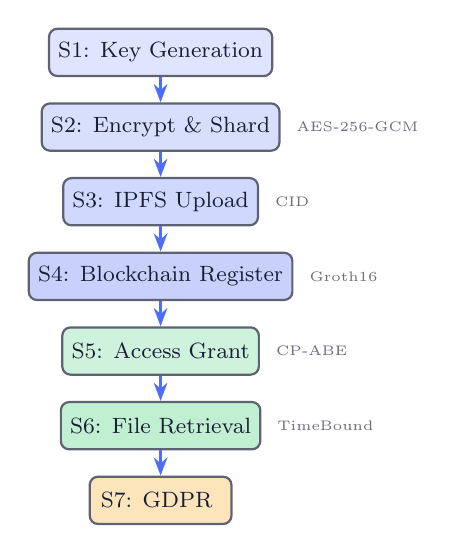
\begin{tikzpicture}[node distance=0.32cm]
  \node[flow, fill=electricblue!18] (s1) {S1: Key Generation};
  \node[flow, fill=electricblue!22, below=of s1] (s2) {S2: Encrypt \& Shard};
  \node[flow, fill=electricblue!27, below=of s2] (s3) {S3: IPFS Upload};
  \node[flow, fill=electricblue!32, below=of s3] (s4) {S4: Blockchain Register};
  \node[flow, fill=successgreen!22, below=of s4] (s5) {S5: Access Grant};
  \node[flow, fill=successgreen!28, below=of s5] (s6) {S6: File Retrieval};
  \node[flow, fill=warnorange!28, below=of s6] (s7) {S7: GDPR };
  \draw[arrow] (s1)--(s2); \draw[arrow] (s2)--(s3);
  \draw[arrow] (s3)--(s4); \draw[arrow] (s4)--(s5);
  \draw[arrow] (s5)--(s6); \draw[arrow] (s6)--(s7);
  \node[right=0.08cm of s2, font=\tiny, text=navyblue!65] {AES-256-GCM};
  \node[right=0.08cm of s3, font=\tiny, text=navyblue!65] {CID};
  \node[right=0.08cm of s4, font=\tiny, text=navyblue!65] {Groth16};
  \node[right=0.08cm of s5, font=\tiny, text=navyblue!65] {CP-ABE};
  \node[right=0.08cm of s6, font=\tiny, text=navyblue!65] {TimeBound};
\end{tikzpicture}
\end{columns}
\end{frame}

\begin{frame}{Cryptographic Pipeline in Detail}
\begin{columns}[t]
\column{0.48\textwidth}
\begin{tcolorbox}[bluebox, title=\textbf{File Encryption (AES-256-GCM)}]
\tiny
\begin{enumerate}
  \item Generate random 256-bit AES key
  \item Split file into \textbf{64\,KB chunks}
  \item Per chunk: 96-bit random IV $\to$ GCM cipher $\to$ auth-tag
  \item SHA-256(plaintext chunk) $\to$ stored integrity hash
  \item Upload encrypted chunks to IPFS $\to$ array of CIDs
  \item Register CIDs + file hash on \texttt{FileRegistry.sol}
\end{enumerate}
\end{tcolorbox}
\vspace{0.12cm}
\begin{tcolorbox}[navybox, title=\textbf{ZKP --- Groth16 Circuits}]
\tiny
\textbf{fileIntegrity.circom:}\\[2pt]
\textbf{Public:} \texttt{fileHash} \\
\textbf{Private:} \texttt{fileChunks[N]}\\
\textbf{Constraint:} $\text{Poseidon(chunks)} = \texttt{fileHash}$
\end{tcolorbox}
\column{0.48\textwidth}
\begin{tcolorbox}[bluebox, title=\textbf{CP-ABE Key Wrapping}]
\scriptsize
\begin{enumerate}
  \item AES key cast to BigInt in BN128 field
  \item Shamir split: threshold = \# policy attributes
  \item Each share encrypted: HKDF(masterKey, attribute) as wrap key
  \item Recipient decrypts shares for their attributes $\to$ reconstruct AES key
\end{enumerate}
\end{tcolorbox}
\vspace{0.12cm}
\begin{tcolorbox}[greenbox, title=\textbf{GDPR Erasure Pipeline}]
\scriptsize
\texttt{requestErasure(fileId)} $\to$ Pinata unpin\\
$\to$ SHA-256 anonymise address in SQLite\\
$\to$ \texttt{isDeleted = true}\\
$\to$ \texttt{fulfillErasure()} on-chain
\end{tcolorbox}
\end{columns}
\end{frame}

% =============================================================================
\section{System Architecture}
% =============================================================================

\begin{frame}{System Architecture --- Four-Layer Stack}
\centering
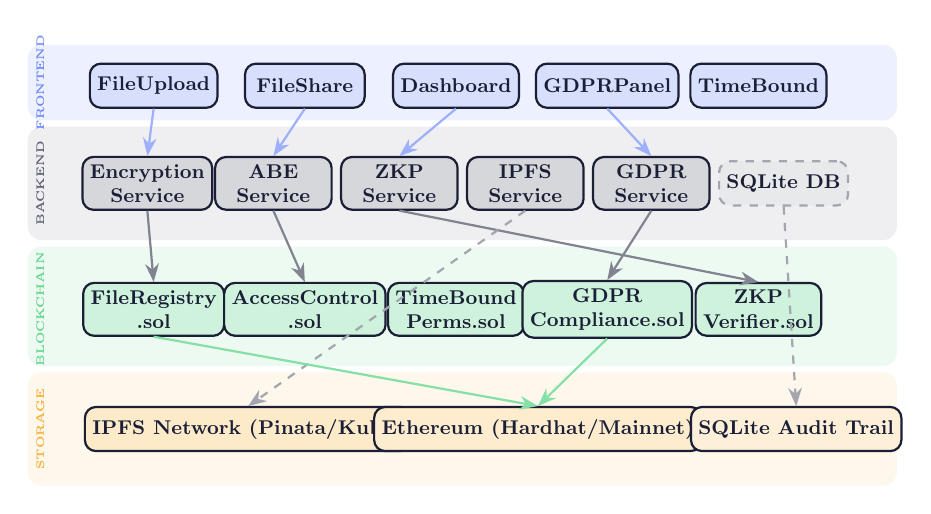
\begin{tikzpicture}[scale=0.80, transform shape]

\begin{scope}[on background layer]
  \fill[electricblue!10, rounded corners=5pt]
    (-0.3,2.2) rectangle (13.5,3.4);
  \fill[navyblue!7, rounded corners=5pt]
    (-0.3,0.3) rectangle (13.5,2.1);
  \fill[successgreen!8, rounded corners=5pt]
    (-0.3,-1.7) rectangle (13.5,0.2);
  \fill[warnorange!8, rounded corners=5pt]
    (-0.3,-3.6) rectangle (13.5,-1.8);
\end{scope}

\node[font=\tiny\bfseries, text=electricblue!80, rotate=90] at (-0.1,2.8) {FRONTEND};
\node[font=\tiny\bfseries, text=navyblue!70, rotate=90]    at (-0.1,1.2) {BACKEND};
\node[font=\tiny\bfseries, text=successgreen!70, rotate=90] at (-0.1,-0.8){BLOCKCHAIN};
\node[font=\tiny\bfseries, text=warnorange!80, rotate=90]  at (-0.1,-2.7){STORAGE};

\node[component, fill=electricblue!22, minimum width=1.9cm] (upload) at (1.7,2.75) {FileUpload};
\node[component, fill=electricblue!22, minimum width=1.9cm] (share)  at (4.1,2.75) {FileShare};
\node[component, fill=electricblue!22, minimum width=1.9cm] (dash)   at (6.5,2.75) {Dashboard};
\node[component, fill=electricblue!22, minimum width=1.9cm] (gdprui) at (8.9,2.75) {GDPRPanel};
\node[component, fill=electricblue!22, minimum width=1.9cm] (tbui)   at (11.3,2.75){TimeBound};

\node[component, fill=navyblue!18, minimum width=1.85cm] (enc)  at (1.6,1.2) {Encryption\\Service};
\node[component, fill=navyblue!18, minimum width=1.85cm] (abe)  at (3.6,1.2) {ABE\\Service};
\node[component, fill=navyblue!18, minimum width=1.85cm] (zkp)  at (5.6,1.2) {ZKP\\Service};
\node[component, fill=navyblue!18, minimum width=1.85cm] (ipfss)at (7.6,1.2) {IPFS\\Service};
\node[component, fill=navyblue!18, minimum width=1.85cm] (gdprs)at (9.6,1.2) {GDPR\\Service};
\node[component, fill=navyblue!10, minimum width=1.7cm,
  draw=navyblue!40, dashed] (db) at (11.7,1.2) {SQLite DB};

\node[component, fill=successgreen!22, minimum width=1.95cm] (fr)  at (1.7,-0.8)  {FileRegistry\\.sol};
\node[component, fill=successgreen!22, minimum width=1.95cm] (ac)  at (4.1,-0.8)  {AccessControl\\.sol};
\node[component, fill=successgreen!22, minimum width=1.95cm] (tbp) at (6.5,-0.8)  {TimeBound\\Perms.sol};
\node[component, fill=successgreen!22, minimum width=1.95cm] (gc)  at (8.9,-0.8)  {GDPR\\Compliance.sol};
\node[component, fill=successgreen!22, minimum width=1.95cm] (zkv) at (11.3,-0.8) {ZKP\\Verifier.sol};

\node[component, fill=warnorange!22, minimum width=3.4cm] (ipfs)   at (3.2,-2.7) {IPFS Network (Pinata/Kubo)};
\node[component, fill=warnorange!20, minimum width=3.4cm] (eth)    at (7.8,-2.7) {Ethereum (Hardhat/Mainnet)};
\node[component, fill=warnorange!16, minimum width=2.4cm] (sqlite) at (11.9,-2.7){SQLite Audit Trail};

\draw[arrow, electricblue!55] (upload.south) -- (enc.north);
\draw[arrow, electricblue!55] (share.south)  -- (abe.north);
\draw[arrow, electricblue!55] (dash.south)   -- (zkp.north);
\draw[arrow, electricblue!55] (gdprui.south) -- (gdprs.north);

\draw[arrow, navyblue!55] (enc.south)  -- (fr.north);
\draw[arrow, navyblue!55] (abe.south)  -- (ac.north);
\draw[arrow, navyblue!55] (zkp.south)  -- (zkv.north);
\draw[arrow, navyblue!55] (gdprs.south)-- (gc.north);

\draw[arrow, navyblue!40, dashed]    (ipfss.south) -- (ipfs.north);
\draw[arrow, navyblue!40, dashed]    (db.south)    -- (sqlite.north);
\draw[arrow, successgreen!55]        (fr.south)    -- (eth.north);
\draw[arrow, successgreen!55]        (gc.south)    -- (eth.north);

\end{tikzpicture}
\end{frame}

% ── Upload & Sharing Workflow ──────────────────────────────────────────────────
\begin{frame}{Upload \& Sharing Workflow}
\centering
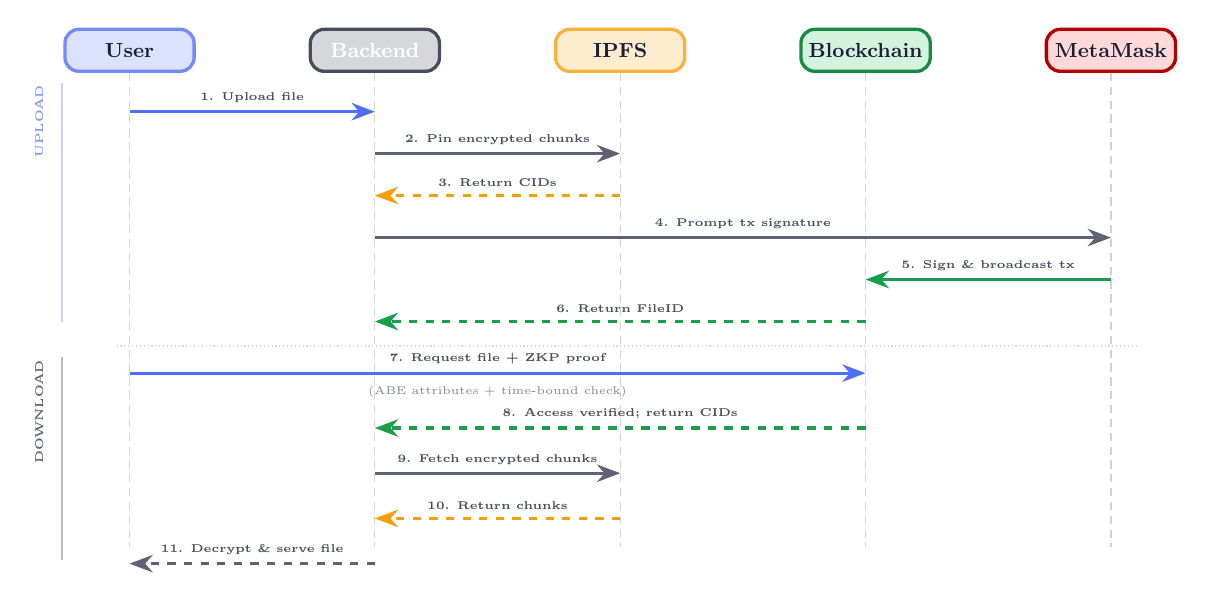
\begin{tikzpicture}[
  actorblue/.style={rectangle, rounded corners=5pt, draw=electricblue!80, very thick,
    fill=electricblue!20, text=navyblue, font=\small\bfseries,
    minimum height=0.65cm, minimum width=2.0cm, align=center},
  actordark/.style={rectangle, rounded corners=5pt, draw=navyblue!80, very thick,
    fill=navyblue!18, text=white, font=\small\bfseries,
    minimum height=0.65cm, minimum width=2.0cm, align=center},
  actororange/.style={rectangle, rounded corners=5pt, draw=warnorange!80, very thick,
    fill=warnorange!20, text=navyblue, font=\small\bfseries,
    minimum height=0.65cm, minimum width=2.0cm, align=center},
  actorgreen/.style={rectangle, rounded corners=5pt, draw=successgreen!70!black, very thick,
    fill=successgreen!20, text=navyblue, font=\small\bfseries,
    minimum height=0.65cm, minimum width=2.0cm, align=center},
  actorred/.style={rectangle, rounded corners=5pt, draw=red!70!black, very thick,
    fill=red!15, text=navyblue, font=\small\bfseries,
    minimum height=0.65cm, minimum width=2.0cm, align=center},
  lbl/.style={font=\tiny\bfseries, text=navyblue!80},
  scale=0.82, transform shape
]

\node[actorblue]   (U)   at (0,0)    {User};
\node[actordark]   (BE)  at (3.8,0)  {Backend};
\node[actororange] (IP)  at (7.6,0)  {IPFS};
\node[actorgreen]  (BC)  at (11.4,0) {Blockchain};
\node[actorred]    (MM)  at (15.2,0) {MetaMask};

\draw[gray!35, densely dashed, thin] (0,-0.35)    -- (0,-7.7);
\draw[gray!35, densely dashed, thin] (3.8,-0.35)  -- (3.8,-7.7);
\draw[gray!35, densely dashed, thin] (7.6,-0.35)  -- (7.6,-7.7);
\draw[gray!35, densely dashed, thin] (11.4,-0.35) -- (11.4,-7.7);
\draw[gray!35, densely dashed, thin] (15.2,-0.35) -- (15.2,-7.7);

\node[font=\tiny\bfseries, text=electricblue!70] at (-1.4,-1.1) {\rotatebox{90}{UPLOAD}};
\draw[electricblue!30, thick] (-1.05,-0.5) -- (-1.05,-4.2);

\draw[-Stealth, very thick, color=electricblue]
  (0,-0.95) -- node[above, lbl] {\textbf{1.} Upload file} (3.8,-0.95);

\draw[-Stealth, very thick, color=navyblue!70]
  (3.8,-1.60) -- node[above, lbl] {\textbf{2.} Pin encrypted chunks} (7.6,-1.60);

\draw[-Stealth, very thick, dashed, color=warnorange]
  (7.6,-2.25) -- node[above, lbl] {\textbf{3.} Return CIDs} (3.8,-2.25);

\draw[-Stealth, very thick, color=navyblue!70]
  (3.8,-2.90) -- node[above, lbl] {\textbf{4.} Prompt tx signature} (15.2,-2.90);

\draw[-Stealth, very thick, color=successgreen!80!black]
  (15.2,-3.55) -- node[above, lbl] {\textbf{5.} Sign \& broadcast tx} (11.4,-3.55);

\draw[-Stealth, very thick, dashed, color=successgreen!80!black]
  (11.4,-4.20) -- node[above, lbl] {\textbf{6.} Return FileID} (3.8,-4.20);

\node[font=\tiny\bfseries, text=navyblue!70] at (-1.4,-5.6) {\rotatebox{90}{DOWNLOAD}};
\draw[navyblue!30, thick] (-1.05,-4.75) -- (-1.05,-7.9);

\draw[gray!30, densely dotted] (-0.2,-4.58) -- (15.6,-4.58);

\draw[-Stealth, very thick, color=electricblue]
  (0,-5.0) -- node[above, lbl] {\textbf{7.} Request file + ZKP proof} (11.4,-5.0);
\node[font=\tiny, text=navyblue!55] at (5.7,-5.28)
  {(ABE attributes + time-bound check)};

\draw[-Stealth, very thick, dashed, color=successgreen!80!black]
  (11.4,-5.85) -- node[above, lbl] {\textbf{8.} Access verified; return CIDs} (3.8,-5.85);

\draw[-Stealth, very thick, color=navyblue!70]
  (3.8,-6.55) -- node[above, lbl] {\textbf{9.} Fetch encrypted chunks} (7.6,-6.55);

\draw[-Stealth, very thick, dashed, color=warnorange]
  (7.6,-7.25) -- node[above, lbl] {\textbf{10.} Return chunks} (3.8,-7.25);

\draw[-Stealth, very thick, dashed, color=navyblue!70]
  (3.8,-7.95) -- node[above, lbl] {\textbf{11.} Decrypt \& serve file} (0,-7.95);

\end{tikzpicture}
\end{frame}

% =============================================================================
\section{Results \& Analysis}
% =============================================================================

\begin{frame}{Results Summary \& Security Analysis}
\begin{columns}[t]
\column{0.48\textwidth}
\begin{tcolorbox}[bluebox, title=\textbf{Smart Contracts Delivered}]
\scriptsize
\begin{itemize}
  \item \texttt{FileRegistry.sol} --- CID storage, soft-delete
  \item \texttt{FileAccessControl.sol} --- ABAC, policy, grant/revoke
  \item \texttt{TimeBoundPermissions.sol} --- auto-expiry, extend
  \item \texttt{GDPRCompliance.sol} --- erasure request \& fulfilment
  \item \texttt{ZKPVerifier.sol} --- Groth16 on-chain verification
\end{itemize}
\end{tcolorbox}
\vspace{0.15cm}
\begin{tcolorbox}[greenbox, title=\textbf{Attack Resistance}]
\scriptsize\centering
51\% attack (PoS/PoA) $\cdot$ DoS resilience $\cdot$ Replay protection
$\cdot$ ReentrancyGuard on all state-changing functions
\end{tcolorbox}
\column{0.48\textwidth}
\begin{tcolorbox}[redbox, title=\textbf{Security Guarantees}]
\scriptsize
\begin{itemize}
  \item \textbf{Confidentiality} --- AES-256-GCM; no plaintext on IPFS
  \item \textbf{Integrity} --- SHA-256 per chunk + ZKP file hash proof
  \item \textbf{Authentication} --- Groth16 ZKP access proof on-chain
  \item \textbf{Authorisation} --- CP-ABE + ABAC (dual layer)
  \item \textbf{Non-repudiation} --- immutable ledger audit trail
  \item \textbf{Privacy} --- ZKP hides attributes; GDPR anonymises PII
  \item \textbf{Availability} --- multi-node IPFS replication (2.8$\times$)
\end{itemize}
\end{tcolorbox}
\end{columns}
\end{frame}

% =============================================================================
\section{Future Work}
% =============================================================================

\begin{frame}{Present Work}
\begin{tcolorbox}[greenbox, title=\textbf{Present Work --- Implemented}]
\small
The system is functional with Basic ZKP, Time-Bound Permissions,
and GDPR compliance fully deployed.
\end{tcolorbox}
\vspace{0.15cm}
\begin{columns}[t]
\column{0.55\textwidth}
\begin{tcolorbox}[bluebox, title=\textbf{Basic ZKP: Data Integrity}]
\scriptsize
\textbf{\texttt{fileIntegrity.circom}}\\[3pt]
\begin{itemize}
  \item Proves encrypted chunks match original file hash
  \item Blockchain verifies file validity \textbf{without seeing content}
  \item Prevents malicious servers from swapping uploaded files
  \item Acts as a \textbf{Trustless Notary} --- focuses on the \textit{Object}
\end{itemize}
\end{tcolorbox}
\column{0.42\textwidth}
\begin{tcolorbox}[greenbox, title=\textbf{Supporting Modules}]
\scriptsize
\begin{itemize}
  \item[\textcolor{successgreen!80!black}{\checkmark}] CP-ABE (Shamir SSS) key encryption
  \item[\textcolor{successgreen!80!black}{\checkmark}] Time-Bound Permissions via \texttt{block.timestamp}
  \item[\textcolor{successgreen!80!black}{\checkmark}] GDPR Art.\ 17 \& 20 hybrid compliance
  \item[\textcolor{successgreen!80!black}{\checkmark}] 5 Solidity contracts + React frontend
\end{itemize}
\end{tcolorbox}
\end{columns}
\end{frame}

\begin{frame}{Future Work}
\begin{tcolorbox}[bluebox, title=\textbf{Future Work --- Planned}]
\small
Priority is Advanced ZKP and to complete CP-ABE for privacy-preserving identity,
followed by production-grade UX enhancements.
\end{tcolorbox}
\vspace{0.15cm}
\begin{columns}[t]
\column{0.55\textwidth}
\begin{tcolorbox}[navybox, title=\textbf{Advanced ZKP: Identity Privacy}]
\scriptsize
\begin{itemize}
  \item Proves user satisfies access policy \textbf{without revealing attributes}
  \item Blockchain sees ``valid user accessed file'' --- never \textit{who} or \textit{why}
  \item Hides role, department, clearance level from public ledger
  \item Acts as a \textbf{Secret Shield} --- focuses on the \textit{Subject}
\end{itemize}
\end{tcolorbox}
\column{0.42\textwidth}
\begin{tcolorbox}[orangebox, title=\textbf{Production UX (Lower Priority)}]
\scriptsize
\begin{itemize}
  \item[\textcolor{warnorange!80!black}{$\circ$}] Google Drive-style interface + drag-and-drop
  \item[\textcolor{warnorange!80!black}{$\circ$}] File versioning, search, bulk operations
  \item[\textcolor{warnorange!80!black}{$\circ$}] ENS name resolution + wallet avatar identity
  \item[\textcolor{warnorange!80!black}{$\circ$}] Expiry countdown timers + toast notifications
\end{itemize}
\end{tcolorbox}
\end{columns}
\end{frame}

% ── Conclusion ────────────────────────────────────────────────────────────────
\begin{frame}{Conclusion}
\begin{tcolorbox}[navybox]
\scriptsize
This work presents a \textbf{fully implemented}, end-to-end decentralised file sharing system that extends
the Blockchain\,+\,IPFS paradigm with \textbf{four novel cryptographic and governance layers}:
\end{tcolorbox}

\vspace{0.06cm}
\begin{columns}[t]
\column{0.48\textwidth}
\begin{tcolorbox}[bluebox, title=\textbf{ZKP}]
\scriptsize Provable identity without credential exposure
\end{tcolorbox}
\vspace{0.06cm}
\begin{tcolorbox}[greenbox, title=\textbf{CP-ABE}]
\scriptsize Policy-driven cryptographic access control
\end{tcolorbox}
\column{0.48\textwidth}
\begin{tcolorbox}[orangebox, title=\textbf{Time-Bound Permissions}]
\scriptsize Self-expiring, blockchain-enforced access rights
\end{tcolorbox}
\vspace{0.06cm}
\begin{tcolorbox}[redbox, title=\textbf{GDPR Module}]
\scriptsize First hybrid Web3 erasure \& export architecture
\end{tcolorbox}
\end{columns}

\vspace{0.08cm}
\begin{tcolorbox}[navybox]
\centering\small
The system provides a \textbf{secure, scalable, legally compliant, and cryptographically verifiable}
foundation for organisations handling sensitive data --- with a clear roadmap toward a
production-ready decentralised storage product.
\end{tcolorbox}
\end{frame}

% ── Thank You Slide ───────────────────────────────────────────────────────────
\begin{frame}[plain]
\begin{tikzpicture}[remember picture, overlay]
  \fill[navyblue] (current page.north west) rectangle (current page.south east);
  \fill[electricblue, opacity=0.18]
    (current page.north east)
    .. controls +(-3,-2) and +(2,2) ..
    ([xshift=-3cm]current page.east)
    -- (current page.south east) -- cycle;
\end{tikzpicture}
\vspace{2.2cm}
\centering
{\Huge\textbf{\textcolor{white}{Thank You}}}\\[0.5cm]


\end{frame}

% =============================================================================
\end{document}